\section{Введение}

Функция (обычно обозначается $y = f(x)$) — это соответствие между двумя множествами, при котором каждому элементу одного множества соответствует \textbf{единственный} элемент другого множества.

\begin{figure}[h]
	\centering
	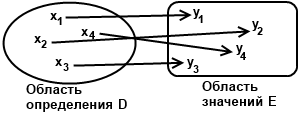
\includegraphics[width=0.5\textwidth]{img/ponyatie-funkcii.png}
	\caption{Понятие функции}
\end{figure}
Допустимые значения аргумента, или \textbf{область определения функции $D(y)$} - это то, что связано с возможными x, при которых функция имеет смысл.

\textbf{Область значений функции $E(y)$} - это то, какие значения принимает y, при допустимых значениях x.

Отсюда следует, что, например, окружность не является функцией.

\begin{figure}[h]
	\centering
	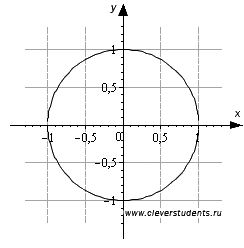
\includegraphics[width=0.3\textwidth]{img/unnamed.png}
	\caption{Здесь одному x (например 0.5) соответствует 2 y}
\end{figure}

\begin{itemize}
    \item x - переменная величина, или, аргумент;
    \item y - зависимая величина – изменяется при изменении аргумента, то есть x согласно какой-либо определенной формуле f, отражающей зависимость одной величины от другой.
\end{itemize}

Далее рассмотрим конструкции элементарных функций.